\documentclass[10pt,twocolumn,uplatex,a4j]{jsreport}
\usepackage{title}
\usepackage{thesis}
\usepackage{abstract}
% \usepackage{balance}

\title{HTML5字句解析仕様の\\自然言語処理による意味解析}
\author{五十嵐彩夏}
\studentid{17B01064}
\department{東京工業大学 情報理工学院 数理・計算科学系}
\supervisor{南出靖彦}
\degree{学士}
\schoolyear{令和2年度}
\submitday{2月5日}

\addtolength{\textwidth}{2cm}
\addtolength{\oddsidemargin}{-1cm}
\addtolength{\evensidemargin}{-1cm}

\pagenumbering{arabic}
\begin{document}
% \setlength{\columnseprule}{0.3pt}
\twocolumn[
\maketitle
]
\section{概要}
HTML5の構文解析を対象とした研究として, 
XSSAuditorの有効性の検証~\cite{XSSAuditor,トランスデューサの包含関係}や, テストの自動生成~\cite{HTML5Testing}などが行われてきた. 
それらの研究は実装段階において, 自然言語によって記述されているHTML5の構文解析仕様から, 手作業でその命令や動作を抽出している. 
このような研究における手作業による翻訳の負担を減らすため, 
本研究では, 自然言語処理を用いて仕様書の命令を自動形式化する. 

本研究の自動形式化の対象である, HTML5字句解析仕様は全て英語によって書かれており, 80個の字句解析の状態の記述で構成されている. 

字句解析の各状態は以下の様に記述されている. 
% 80個の状態のあるオートマトンとして定義されており, 
% \noindent
% Emit a U+003C LESS-THAN SIGN character token. Reconsume in the RCDATA state.
\begin{quote}
13.2.5.9 RCDATA less-than sign state\\
Consume the next input character:\\
$\hookrightarrow$U+002F SOLIDUS (/)\\
\ Set the temporary buffer to the empty string.\\
\ Switch to the RCDATA end tag open state.\\
$\hookrightarrow $Anything else\\
\ $\cdots\ $
\end{quote}

% HTML5字句解析仕様の記述内容をもとに, 
% その仕様記述言語を以下の型として定義した. %
% \begin{description}
%     \item[Command] 命令文を表現する型
%     \item[Bool] 条件分岐文の条件部分を表現する型
%     \item[CommandValue] 字句解析仕様の変数や値を表現する型
%     \item[InplementVariable] 字句解析仕様の代入される変数を表現する型
% \end{description}
% それぞれの型が有する値は仕様書に出てくる文や語句に基づいて定める. 
% 例えば, Command型には以下のような値を持つ. 

字句解析仕様の記述内容をもとに, 以下のような命令を持つ仕様記述言語を定義する. 
% \begin{alignat*}{3}
%     \mbox{ Command }::&= &\quad&\mbox{ If } &\quad&\mbox{ // 条件分岐文} \\ 
%       &|& &\mbox{ Switch } & &\mbox{ // 状態遷移命令} \\
%       &|& &\mbox{ Create } & &\mbox{ // 新しくトークンを作る命令 } \\
%       &|& &\mbox{ Set } & &\mbox{ // 値の代入の命令} \\
%       &|& & \cdots & & \\
% \end{alignat*}
\begin{alignat*}{3}
    \mbox{ command }::&= &\ &\mbox{ If(bool, commandList$_1$, commandList$_2$)} &&\\
      &|& &\mbox{ Switch(cVal)} & &\\
    %   &|& &\mbox{ Create(string, cVal)} & &\\
      &|& &\mbox{ Set(iVal, cVal)} & & \\
      &|& &\mbox{ Emit(cVal)} & &\\
      &|& & \cdots & & 
\end{alignat*}

例えば, Ifは条件分岐文, Switchは字句解析の状態の遷移命令, Setは変数iValに値cValを代入する命令を表している. 
(boolは条件文を表す値, commandListは命令のリストを表す値, cVal, iValは字句解析器の変数や値を表す値)

上記の字句解析の状態のU+002F SOLIDUS (/)の部分を仕様記述言語のプログラムへ変換すると, 
以下のようになる. 
\begin{quote}
Set(ITemporaryBuffer, CString()), \\
Switch(StateName(RCDATA end tag open state)) 
\end{quote}

% Set, SwitchはCommand型の値で, 
% CStringは文字列を引数に持つCommandValue型の値, 
ITemporaryBuffer字句解析の一時バッファという変数という意味の値, 
StateNameは状態名を引数に持つ, 字句解析状態名という意味の値である. \\


本研究では, まず, 自然言語処理のライブラリであるStanford CoreNLP~\cite{manning-EtAl:2014:P14-5}を使い, HTML5の字句解析仕様に対して自然言語処理を適用する. 
その際, 自然言語処理そのまま適用するのではなく, 前処理として特定の文字列の置き換えを導入する. 
そして, 自然言語処理による構文解析や意味解析の結果を使い, 構文解析木に単語の原型や参照関係の情報を付加したデータ型へ変換する. 
更にそのデータ型から木構造のマッチングを用いて仕様記述言語の仕様に変換する. 
最後に, 字句解析のインタプリタを作成し, それをもとにHTML5の字句解析のテストを行い, 正しく仕様記述言語へ変換出来たことを確認する. 

% また, 構文木解析の結果を用いて命令を抽出する際も, 条件分岐文のスコープを人の手で判断するように作るなど, 命令の抽出の仕方に関する工夫を行った. 

% \section{HTML5字句解析仕様の自動形式化}

% 以下でその変換過程について説明をする. 

% \section{仕様記述言語}
% HTML5字句解析の仕様記述言語を以下の型として定義した. 
% \begin{description}
%     \item[Command] 命令文を表現する型
%     \item[Bool] 条件分岐文の条件部分を表現する型
%     \item[CommandValue] 字句解析仕様の変数や値を表現する型
%     \item[InplementVariable] 字句解析仕様の代入される変数を表現する型
% \end{description}
% それぞれの型が有する値は仕様書に出てくる文, 語句に基づいて定めた. 

\section{仕様への自然言語処理の適用}
自然言語処理ライブラリStanford CoreNLPを使い, HTML5字句解析仕様に対して自然言語処理を適用する. 
そして, 構文解析木, それぞれの単語の原型, 文の語句間の参照関係の情報を取り出す. 
それらの情報を, Scalaのデータ型として定義した, 
構文解析木に単語の原型と参照関係の情報を付加した型である, \texttt{Tag}型に変換する. 

例えば, ``Mika likes her dog''という文章に対して, 
自然言語処理を適用すると, \\
単語の原型がそれぞれ, 
Mika,  like,   she,   dog 
であることが分かり, 
また, Mikaとherにラベルが1の参照関係が存在することが分かる. 

そして構文解析木は以下の左図のようになり, 
これらの情報から, 右図のようなTag型の値に変換される. 
\begin{figure}[H]
    \centering
    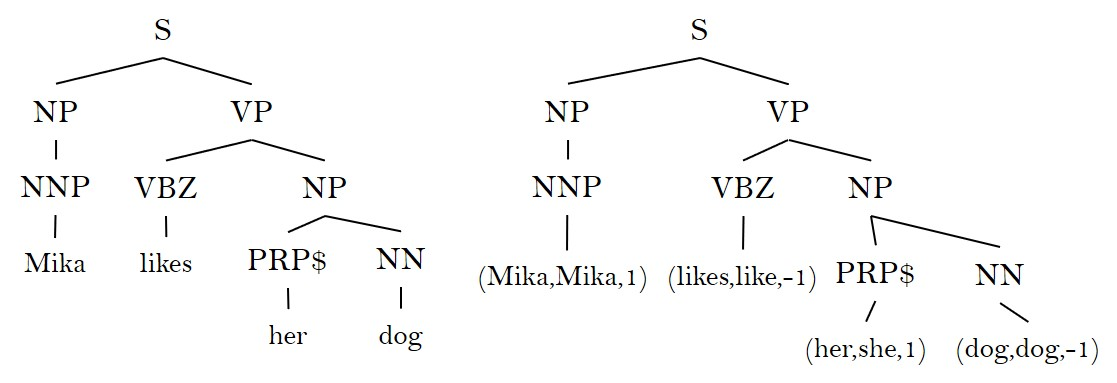
\includegraphics[keepaspectratio, scale=0.46]
         {tree.jpg}
\end{figure}

しかし, 字句解析仕様の文に対してそのまま自然言語処理を適用すると, トークンの分割や品詞解析が適切な形で解釈されない場合がある. 

そのため自然言語処理する際に前処理として, 特定の文字列の置き換えをし, 適切に文章が解釈されるようにする. 

% \subsection{前処理:文字列の置き換え}
% 自然言語処理したい文章をそのまま処理すると, トークンの分割や品詞解析が適切な形で解釈されない場合がある. 
% よって, 自然言語処理する際に前処理として, 特定の文字列の置き換えをし, 適切に文章が解釈されるようにする. 
例えば, 以下のような置き換えを行う. 
\begin{itemize}
    \item 状態名を1つのトークンとして認識させるため, 字句解析の状態名を表す語句に対して, 空白 及び ``\texttt{-}'' を ``\texttt{_}'' に置き換える. ``('' , ``)'' を除く. 先頭を大文字にする.
    \item ユニコード``U+xxxx''を1つのトークンとして認識させるため, ``+''を``\_''に置き換える. 
    \item 命令文の解釈が上手くいくように, ``Reconsume''など自然言語の解釈が上手くいかない動詞の前に仮の主語を表す``you'' を加える. 
    % \item 命令文の解釈が上手くいくように, 一部の動詞を表す文字列 ``Switch'', ``Reconsume'', ``Emit'', ``Flush'', ``Append'', ``Add'', ``Multiply'' の前に``you'' を加える. %特定の動詞の前
    % \item ``-''で繋がれている単語は1つのトークンとして認識されないため, ``-'' を ``_''に置き換える.
    % \item 句読点をまたいでいる場合,参照関係の解析が上手くいかないことがあったので, 参照関係が多く出てくるSet文に関して, 
    % ``(,$|$.) set'' $\Rightarrow$ `` and set'' と置き換える.
    % \item ``!''が文末記号と認識されるため, ``!'' は ``EXC'' に置き換える.
 \end{itemize}
% \subsection{自然言語処理の適用}
% 仕様書の文字の置き換えの前処理を行った文に, 自然言語処理ライブラリStanford CoreNLPを使い自然言語処理を適用する. 
% そして, 構文解析木, それぞれの単語の原型, 文中の語句の参照関係の情報を取り出す. 
% \subsection*{データ型\texttt{Tag}への変換}
% % 自然言語処理での出力をもとに, 
% % Scalaのデータ型として定義した, 構文解析木に原型や参照関係の情報を付加した型である, \texttt{Tag}型の値へ変換する. 
% 自然言語処理で得た結果を, 
% Scalaのデータ型として定義した, 
% 構文解析木に単語の原型と参照関係の情報を付加した型である, \texttt{Tag}型に変換する. %の葉の部分

\section{仕様記述言語への変換}
自然言語処理で得た\texttt{Tag}型から, 
\texttt{Tag}型のパターンマッチングを用いて, 仕様記述言語への変換を行う. 

\texttt{Tag}型の値が文, 動詞句を表す場合は, 
変換元の代表的な文の構文木の形を調べ, それに基づいた %変換の規則は, Tag型の値のパターンマッチを作る.
パターンマッチを行うプログラムを作成する. それに応じて変換をする. 

\texttt{Tag}型の値が名詞句を表す場合は単純に特定の文字列が含まれているかを判断し, それに応じて変換をする. 
% 例えば, 
% \subsection*{文を表現するTag型の値からCommand型の値のリストへの変換}
% \texttt{Tag}型の値から仕様記述言語の型の値への変換を関数として表現した. 
% \begin{description}
%     \item[$\mathcal{T}_S$] 文を表現するTag型の値からCommand型の値のリストへ変換する
%     \item[$\mathcal{T}_B$] 条件文を表現するTag型の値からBool型の値へ変換する関数
%     \item[$\mathcal{T}_{VP}$] 動詞句を表現するTag型の値からCommand型の値のリストへ変換する関数
%     \item[$\mathcal{D}$] 複数の名詞が含まれている名詞句を表現するTag型の値を1つの単位の名詞句を表現するTag型の値に分割する関数
%     \item[$\mathcal{T}_{NP_{C}}$] 名詞句を表現するTag型の値からCommandValue型の値へ変換する関数
%     \item[$\mathcal{T}_{NP_{I}}$] 名詞句を表現するTag型の値からImplementVariable型の値へ変換する関数
% \end{description}
% $\mathcal{T}_{NP_{C}}$と$\mathcal{T}_{NP_{I}}$に関しては, 単純に特定の文字列が含まれているかどうかで変換する対象を決める. 

\subsection*{条件分岐文の処理}
仕様書には, ``If $\cdots$ ,then $\cdots$ . Otherwise $\cdots$ .''のような条件分岐文も含まれる. 
その際, 条件文のスコープ(Otherwiseで処理する部分)が明らかでない場合がある. %条件がFlaseの場合の処理が文書のどの文までなのかが明らかでない

よって, 仕様記述言語への変換の際に, 
そのようなものがあったら, 変換の途中で人の手でスコープを選ぶようにする. 

\section{字句解析のテスト}
プログラミング言語Scalaで仕様記述言語のインタプリタを作成した. %HTML5の字句解析
そして, 仕様記述言語のインタプリタと, 自然言語処理によって形式化した字句解析仕様をもとに, HTML5の字句解析器を実装した. 

% から形式化した仕様記述言語のプログラムの正しさを
字句解析仕様から抽出した命令の正しさを検証するため, HTML5の字句解析のテストデータを使い, 字句解析器のテストを行った. 

テストを行った結果, 6,574/7,029個のテストが成功した. 
これは, 文字の置き換えの前処理を行ったことや, \texttt{Tag}型の構文木の変換において, いくつかの文章にアドホックな対応をしたことから, 上手くいったと考えられる. 

しかし, 失敗した部分の原因について, 適切に命令を抽出できたと見えても, 実際は正しいものから少しずれていたというケースがあった. %り, 失敗したものがあった. 
それに対してアドホックな形で字句解析インタプリタの処理に対する対処をしたら, 全てのテストが成功した. 

% 例えば字句解析の状態``After DOCTYPE name state''において, 入力文字列が``public $\cdots$''であるとき, 
% まず文字`p'を消費し, その文字マッチングによりAnything elseの処理を行う. 
% その処理の文の中の``If the six characters starting from the current input character are an ASCII case-insensitive match for the word ``PUBLIC'', then consume those characters''の部分において, 
% これを形式化すると, $[\ $If(AsciiCaseInsensitiveMatch(Substitute(``1'', CharactersFromCurrentInputCharacter(6)), CString(``PUBLIC''))), Comsume(Variable(``1''))$\ ]$となので, 
% この処理を行うとき, 変数``1''は``public''という文字列を指すことになる. よってComsume(Variable(``1''))は文字列``public''を消費するという操作になる. 

% しかし, この時入力文字列が``ublic $\cdots$''という状態であるはずだから, 適切に処理をするために本来は文字列``ublic''を消費すべきである. 
% このように, 人間なら``those characters''の指しているものをそのまま消費すると上手くいかないとわかることを, 機械だとうまく認識できないという問題が見られた. 

% この問題に対して, 
% 字句解析インタプリタのConsume文の処理において, 消費したい文字列が入力文字列の最初の部分に一致してないと消費することが出来ない部分を, 
% 現在消費した文字+入力文字列の最初の部分に一致していたら, 入力文字列にあたる部分のみを消費できるようにする
% という形で対応をした. 

% \section{結論}
% 本研究では, HTML5の字句解析仕様に対して, 命令の形式化を行い, そして自然言語処理の適用をし, 
% その単語と構文木, 参照関係の解析結果を用いることで, 命令の自動形式化を行った. 
% そして, 字句解析のインタプリタを作成し, HTML5の字句解析のテストを行い, 正しく命令の抽出が出来たことを確認できた. 

% しかし, 
% \texttt{Tag}型から仕様記述言語への変換において, 構文木が特殊な形である場合に個別に対応する必要出てきたり, 
% 名詞句のTag型の値からCommandValue型への変換が単に文字列のマッチングをするという愚直なやり方になってしまった部分がある. 

% よって, 自然言語処理の適用において, 係り受け解析(dependency parse)の情報の利用も検討したい. 
\bibliographystyle{plain}
\bibliography{thesis}
\end{document}